\documentclass[conference]{IEEEtran}
\IEEEoverridecommandlockouts
\usepackage{cite}
\usepackage{amsmath,amssymb,amsfonts}
\usepackage{algorithmic}
\usepackage{graphicx}
\usepackage{textcomp}
\usepackage{xcolor}
\usepackage{booktabs}
\usepackage{float}

\begin{document}

\title{Comparative Analysis of Naive Bayes and Convolutional Neural Networks for Automated PCOS Detection from Ultrasound Imagery}

\author{
\IEEEauthorblockN{Gauri Deshmukh}
\IEEEauthorblockA{\textit{B.Tech Data Science} \\
\textit{MPSTME, NMIMS}\\
}
}

\maketitle

\begin{abstract}
Polycystic Ovary Syndrome (PCOS) is a common hormonal disorder among women of reproductive age. Early and accurate detection through ultrasound imagery is very important for effective treatment. However, manually interpreting these ultrasound images can be subjective and prone to human error. In this project, we built an automated computer program to classify ovarian ultrasound images into 'Normal' and 'Abnormal' (showing PCOS) categories. We compared two different machine learning methods: a traditional Gaussian Naive Bayes model and a more advanced Convolutional Neural Network (CNN). Both models were trained and tested on a custom dataset of ultrasound images. We evaluated their performance using Accuracy, Precision, Recall, and F1-Score. Our results show that the CNN, which automatically learns spatial patterns in images, significantly outperforms the simpler Naive Bayes model, making it a much more reliable tool for medical diagnosis.
\end{abstract}

\begin{IEEEkeywords}
Polycystic Ovary Syndrome (PCOS), Ultrasound Imaging, Convolutional Neural Networks (CNN), Naive Bayes, Machine Learning, Deep Learning, Medical Image Classification, Computer-Aided Diagnosis.
\end{IEEEkeywords}

\section{Introduction}
Polycystic Ovary Syndrome (PCOS) is widely recognized as one of the most common endocrinopathies affecting 6\% to 20\% of women of reproductive age globally, depending on the diagnostic criteria employed. The syndrome is clinically defined by a heterogeneous presentation of hyperandrogenism, ovulatory dysfunction, and the presence of polycystic ovarian morphology (PCOM) visible on transvaginal or transabdominal ultrasound scans. According to the internationally recognized Rotterdam criteria established in 2003, a definitive diagnosis of PCOS requires the presence of at least two of these three clinical features. Because ovarian morphology is a critical pillar of this diagnostic triad, ultrasound imaging serves as a frontline modality in gynecological examinations. 

A typical polycystic ovary is characterized by the presence of 12 or more follicles measuring 2-9 mm in diameter, often arranged peripherally (the "string of pearls" sign), and an increased ovarian volume (typically $>$ 10 cm$^3$). However, identifying and quantifying these sub-centimeter cystic structures within the noisy, low-contrast environment typical of ultrasound imagery presents a formidable challenge. Manual assessment is highly susceptible to inter-observer and intra-observer variability. Fatigue, variations in ultrasound equipment quality, and the sheer volume of diagnostic imaging in clinical settings further exacerbate the potential for misinterpretation.

To address these challenges, the medical imaging community has increasingly turned towards Computer-Aided Diagnosis (CAD) systems powered by Artificial Intelligence (AI). The primary objective of these systems is not to replace the radiologist but to serve as an objective, highly sensitive secondary screening tool. In recent years, both traditional machine learning (ML) algorithms and deep learning (DL) models have been applied to this domain. Traditional ML approaches often rely on hand-crafted feature extraction techniques—such as Gray-Level Co-occurrence Matrices (GLCM), Local Binary Patterns (LBP), or direct pixel intensity distributions—followed by classifiers like Support Vector Machines (SVM), Random Forests, or Naive Bayes. While computationally inexpensive, these methods struggle to capture the complex, non-linear spatial dependencies inherent in anatomical structures.

Conversely, Deep Learning, particularly Convolutional Neural Networks (CNNs), has revolutionized medical image analysis. CNNs automatically learn hierarchical feature representations directly from raw pixel data, progressively abstracting simple edges and textures into complex structural representations. By preserving the 2D spatial topology of the image, CNNs are exceptionally well-suited for identifying the subtle morphological anomalies characteristic of PCOS.

In this research, we conduct a rigorous comparative analysis between these two dichotomous approaches. We implement a Gaussian Naive Bayes classifier as a representative of traditional probabilistic modeling. We contrast this against a custom-designed CNN architecture. By evaluating these models on the identical dataset, we aim to systematically quantify the performance gap between pixel-wise independence assumptions and deep spatial feature learning, providing mathematical justifications and comprehensive empirical evidence.

\section{Literature Review}
The application of computational intelligence to PCOS diagnosis has seen significant growth over the past decade. Early attempts primarily focused on clinical, biochemical, and demographic data. For instance, researchers utilized Support Vector Machines (SVM) and multi-layer perceptrons to classify PCOS based on hormonal profiles (e.g., Luteinizing Hormone (LH), Follicle-Stimulating Hormone (FSH), testosterone). 

In the realm of ultrasound image analysis, traditional approaches heavily relied on manual or semi-automated segmentation. Initial studies employed edge detection algorithms and morphological operations to isolate ovarian borders and individual follicles. Extracted features were then fed into classifiers. While these methods demonstrated proof-of-concept, they were highly sensitive to image noise (speckle) and required extensive parameter tuning for different ultrasound machines.

The paradigm shift occurred with the advent of Deep Learning. Several studies have recently applied CNNs to PCOM detection. Transfer learning, utilizing networks pre-trained on the ImageNet dataset such as ResNet-50, VGG-16, and InceptionV3, has become a popular methodology. For example, some researchers have achieved accuracies exceeding 85\% by fine-tuning deep networks on relatively small ovarian ultrasound datasets. Other approaches have utilized object detection frameworks like YOLO (You Only Look Once) or Mask R-CNN to not only classify the image but to explicitly localize and count individual follicles.

Despite these advancements, many existing studies rely on highly curated, heavily pre-processed datasets, often failing to compare the efficacy of deep learning against robust traditional baselines under identical, minimally pre-processed conditions. This study seeks to bridge that gap by providing a foundational comparison, emphasizing the mathematical mechanisms that drive the observed performance disparities between a Gaussian Naive Bayes approach and a bespoke CNN.

\section{Methodology}

\subsection{Dataset Information}
The empirical foundation of this study is a custom-curated dataset of ovarian ultrasound images. The images exhibit varying degrees of noise, resolution, and contrast, representative of real-world clinical environments. The dataset is partitioned into a labeled training set and an unlabeled test set for blind prediction. The ground truth labels, denoted by the target variable $y$, represent a binary classification task based on the `abnormality` or `pcos\_visible` status:
\begin{itemize}
    \item \textbf{Class 0 ($y=0$):} Normal ovarian morphology.
    \item \textbf{Class 1 ($y=1$):} Abnormal morphology, indicative of Polycystic Ovary Syndrome (PCOS).
\end{itemize}
The training dataset comprises 3,200 images, exhibiting a class imbalance typical in medical datasets: 903 images are categorized as Normal, and 2,297 as Abnormal. The test dataset contains 1,468 images.

\begin{figure}[H]
    \centering
    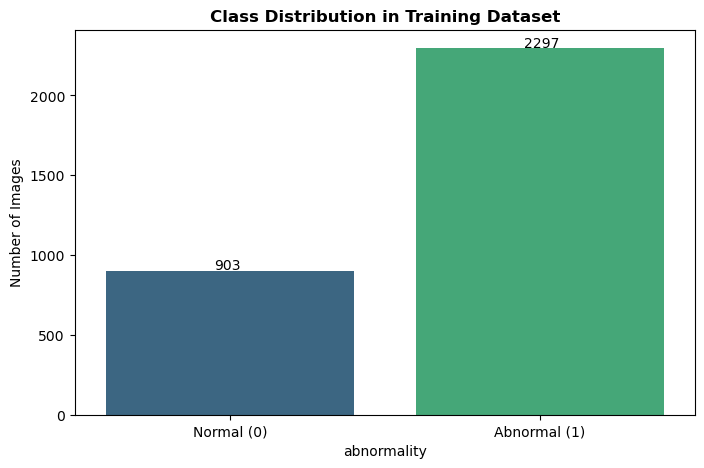
\includegraphics[width=0.48\textwidth]{graph_cell_4_0.png}
    \caption{Class Distribution in the Training Dataset, highlighting the categorical imbalance between Normal and Abnormal (PCOS) morphologies.}
    \label{fig:class_dist}
\end{figure}

\subsection{Image Preprocessing}
Given the computational complexity of image processing, standardization of the input data is a critical prerequisite. The preprocessing pipeline consists of three sequential operations:
\subsubsection{Grayscale Conversion}
Ultrasound images inherently capture structural density rather than true color information. Therefore, images are converted to single-channel grayscale arrays. Let an image be represented by a matrix $\mathbf{I} \in \mathbb{R}^{H \times W \times 3}$. The grayscale transformation is defined as a weighted linear combination of the Red (R), Green (G), and Blue (B) channels to match human luminance perception:
\begin{equation}
    Y(i,j) = 0.299 \cdot R(i,j) + 0.587 \cdot G(i,j) + 0.114 \cdot B(i,j)
\end{equation}
where $Y(i,j)$ is the resulting grayscale intensity at pixel coordinates $(i,j)$.

\subsubsection{Resizing}
To facilitate batch processing through fixed-architecture neural networks, all images are resized to a uniform spatial dimension of $128 \times 128$ pixels using bi-linear interpolation. Thus, the input vector space $\mathbf{x}$ for any given image belongs to $\mathbb{R}^{128 \times 128}$.

\subsubsection{Normalization and Tensor Flattening}
For the Naive Bayes classifier, the 2D spatial structure is discarded. The image matrix is flattened into a 1D vector $\mathbf{x} \in \mathbb{R}^{d}$, where $d = 128 \times 128 = 16,384$ features. To optimize the convergence and performance of the probabilistic estimator, the feature vectors are standardized to achieve a mean of zero and a standard deviation of one (Z-score normalization). For a feature vector $\mathbf{x} = [x_1, x_2, \dots, x_d]^T$, the standardized value $x_i'$ is given by:
\begin{equation}
    x_i' = \frac{x_i - \mu_i}{\sigma_i}
\end{equation}
where $\mu_i$ is the empirical mean and $\sigma_i$ is the empirical standard deviation of the $i$-th pixel across the entire training corpus.

\begin{figure}[H]
    \centering
    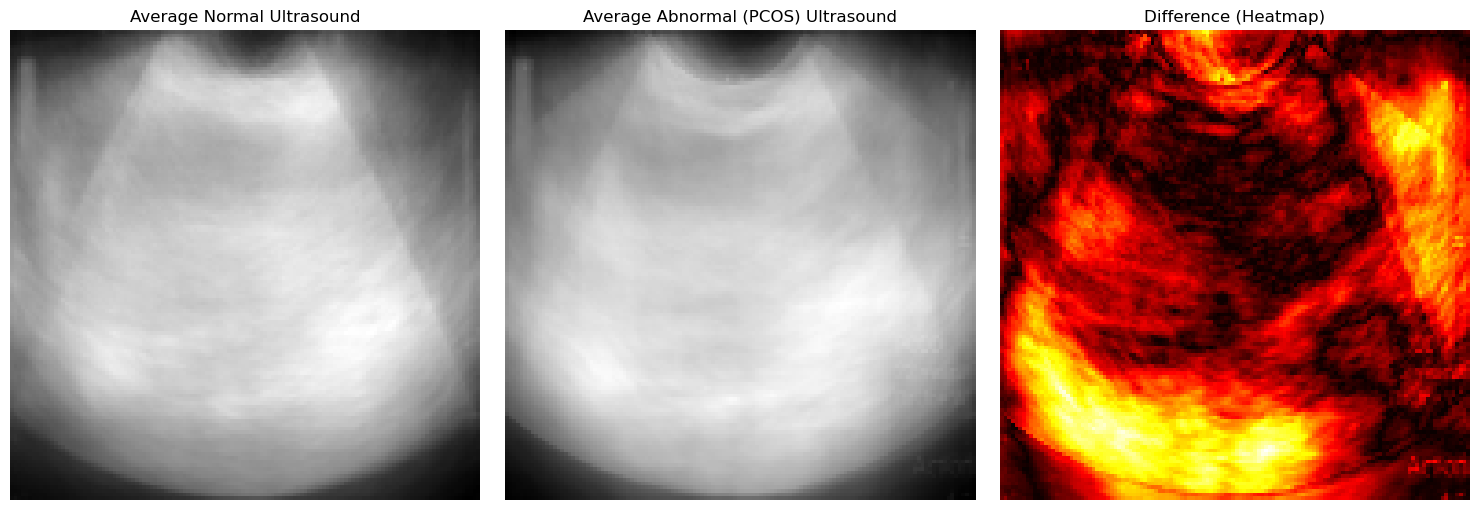
\includegraphics[width=0.48\textwidth]{graph_cell_10_2.png}
    \caption{Visual structural comparison: Average Normal Ultrasound, Average Abnormal (PCOS) Ultrasound, and the resulting Structural Difference Heatmap. The heatmap exposes subtle regions of morphological variance corresponding to follicular distributions.}
    \label{fig:heatmap}
\end{figure}

\begin{figure}[H]
    \centering
    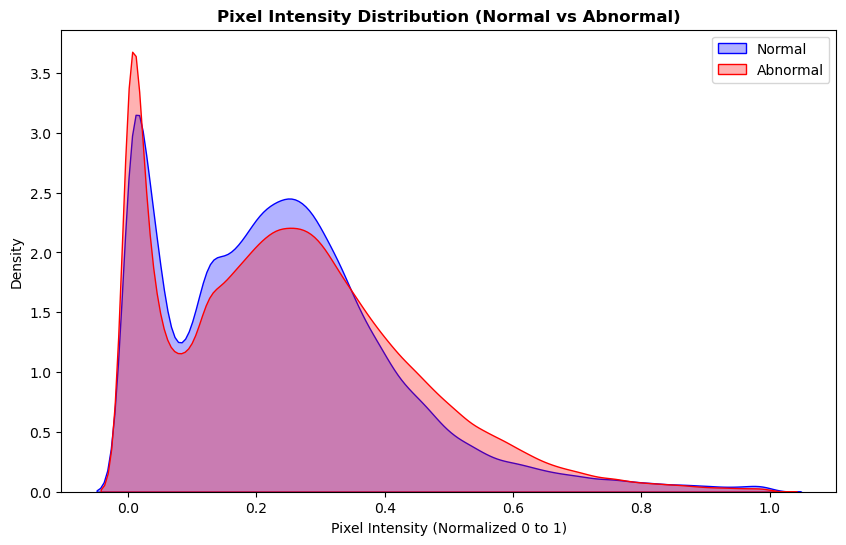
\includegraphics[width=0.48\textwidth]{graph_cell_12_3.png}
    \caption{Kernel Density Estimation of Pixel Intensity Distributions across Normal and Abnormal classes. The significant overlap demonstrates non-linear structural complexities that severely complicate baseline probabilistic classification.}
    \label{fig:intensity}
\end{figure}

\subsection{Gaussian Naive Bayes Model}
The Naive Bayes classifier is a probabilistic machine learning model based on Bayes' Theorem. It is "naive" because it makes the strong, often unrealistic, assumption that the features (pixel intensities) are conditionally independent given the class label.

According to Bayes' Theorem, the posterior probability of a class $C_k$ (where $k \in \{0, 1\}$) given an input feature vector $\mathbf{x} = (x_1, x_2, \dots, x_d)$ is formulated as:
\begin{equation}
    P(C_k | \mathbf{x}) = \frac{P(C_k) \cdot P(\mathbf{x} | C_k)}{P(\mathbf{x})}
\end{equation}
Here, $P(C_k)$ is the prior probability of class $C_k$, $P(\mathbf{x} | C_k)$ is the likelihood, and $P(\mathbf{x})$ is the marginal likelihood (evidence). Under the naive independence assumption, the joint likelihood factors into the product of individual marginal likelihoods:
\begin{equation}
    P(\mathbf{x} | C_k) = \prod_{i=1}^{d} P(x_i | C_k)
\end{equation}
Because the input features $x_i$ are continuous real-valued pixel intensities, we model their likelihood using a Gaussian (Normal) distribution. Thus, the probability density function for a feature $x_i$ given class $C_k$ is:
\begin{equation}
    P(x_i | C_k) = \frac{1}{\sqrt{2\pi\sigma_{ki}^2}} \exp\left( - \frac{(x_i - \mu_{ki})^2}{2\sigma_{ki}^2} \right)
\end{equation}
where $\mu_{ki}$ and $\sigma_{ki}^2$ are the mean and variance of feature $x_i$ associated with class $C_k$, estimated from the training data. The classifier assigns the input $\mathbf{x}$ to the class $\hat{y}$ that maximizes the Maximum A Posteriori (MAP) decision rule:
\begin{equation}
    \hat{y} = \arg\max_{k \in \{0, 1\}} P(C_k) \prod_{i=1}^{d} P(x_i | C_k)
\end{equation}
In practice, to prevent numerical underflow associated with multiplying many small probabilities, the log-likelihood is computed instead:
\begin{equation}
    \hat{y} = \arg\max_{k \in \{0, 1\}} \left( \ln P(C_k) + \sum_{i=1}^{d} \ln P(x_i | C_k) \right)
\end{equation}

\subsection{Convolutional Neural Network (CNN) Model}
While Naive Bayes treats pixels as independent entities, CNNs are explicitly designed to process data with a known grid-like topology, exploiting local spatial correlations. Our proposed custom architecture consists of sequential convolutional blocks followed by fully connected dense layers.

\subsubsection{Convolutional Layers}
The core building block of a CNN is the convolutional layer. A 2D convolution operation applies a set of learnable filters (kernels) across the input image. For an input feature map $X$ and a filter $K$ of size $m \times n$, the output feature map $Y$ at spatial location $(i, j)$ is computed as:
\begin{equation}
    Y(i, j) = (X * K)(i, j) = \sum_{u=0}^{m-1} \sum_{v=0}^{n-1} X(i+u, j+v) \cdot K(u, v)
\end{equation}
Our architecture utilizes $3 \times 3$ kernels. The depth of the feature maps progressively increases through four convolutional layers (32, 64, 128, and 256 filters, respectively), allowing the network to learn increasingly complex structural representations of the ovarian tissue.

\subsubsection{Activation Function}
To introduce non-linearity into the network, enabling it to learn complex mappings, the Rectified Linear Unit (ReLU) activation function is applied element-wise to the output of each convolutional layer:
\begin{equation}
    f(x) = \max(0, x)
\end{equation}
ReLU mitigates the vanishing gradient problem commonly encountered in deep networks during backpropagation.

\subsubsection{Max Pooling Layers}
To achieve spatial invariance and reduce computational burden, $2 \times 2$ Max Pooling layers follow each convolutional layer. The pooling operation downsamples the feature map by selecting the maximum value within a defined window. For a $2 \times 2$ window with stride 2, the output $Y$ is:
\begin{equation}
    Y(i, j) = \max_{u \in \{0, 1\}, v \in \{0, 1\}} X(2i+u, 2j+v)
\end{equation}

\subsubsection{Batch Normalization}
To accelerate convergence and stabilize the learning process, Batch Normalization is employed after each pooling operation. It normalizes the activations of the previous layer over the mini-batch to have zero mean and unit variance, followed by applying a learnable scale $\gamma$ and shift $\beta$:
\begin{equation}
    \hat{x_i} = \frac{x_i - \mu_{\mathcal{B}}}{\sqrt{\sigma_{\mathcal{B}}^2 + \epsilon}}
\end{equation}
\begin{equation}
    y_i = \gamma \hat{x_i} + \beta
\end{equation}
where $\mu_{\mathcal{B}}$ and $\sigma_{\mathcal{B}}^2$ are the mini-batch mean and variance, and $\epsilon$ is a small constant for numerical stability.

\subsubsection{Fully Connected Layers and Dropout}
The 2D feature maps from the final convolutional block are flattened into a 1D vector $\mathbf{a}^{(0)}$ and fed into two dense (fully connected) layers containing 256 and 128 neurons, respectively. The forward pass for a dense layer $l$ computes the affine transformation followed by the ReLU activation $f$:
\begin{equation}
    \mathbf{a}^{(l)} = f(\mathbf{W}^{(l)} \mathbf{a}^{(l-1)} + \mathbf{b}^{(l)})
\end{equation}
where $\mathbf{W}^{(l)}$ is the weight matrix and $\mathbf{b}^{(l)}$ is the bias vector for layer $l$. 

To combat overfitting, Dropout regularization is applied with a rate of $p=0.5$. Dropout temporarily deactivates a random subset of neurons during training, forcing the network to learn redundant and robust features. For a given neuron output $y_j$:
\begin{equation}
    r_j \sim \text{Bernoulli}(1-p)
\end{equation}
\begin{equation}
    \tilde{y}_j = r_j \cdot y_j
\end{equation}

\subsubsection{Output Layer}
The final dense layer contains 2 neurons corresponding to the two classes. The Softmax activation function converts the raw logits $\mathbf{z}$ into normalized probability distributions:
\begin{equation}
    P(y = k | \mathbf{x}) = \frac{e^{z_k}}{\sum_{j=0}^{1} e^{z_j}} \quad \text{for } k \in \{0, 1\}
\end{equation}

\section{Implementation Infrastructure}
The experiments were conducted using the Python programming language, utilizing Scikit-learn for the Naive Bayes implementation and TensorFlow/Keras for the Deep Learning architecture. 

\subsection{Loss Function and Optimization}
The CNN was trained to minimize the Sparse Categorical Cross-Entropy loss function, which quantifies the divergence between the predicted probability distribution and the true label. For a single observation with true class $y \in \{0, 1\}$ and predicted probability $p_y$, the loss $\mathcal{L}$ is:
\begin{equation}
    \mathcal{L} = - \sum_{k=0}^{1} \delta(y, k) \log(p_k)
\end{equation}
where $\delta(y, k)$ is the Kronecker delta (1 if $y=k$, 0 otherwise).

Optimization was performed using the Adam (Adaptive Moment Estimation) algorithm. Adam dynamically adjusts the learning rate for each parameter by computing exponential moving averages of the gradient $m_t$ (first moment) and the squared gradient $v_t$ (second moment):
\begin{equation}
    m_t = \beta_1 m_{t-1} + (1 - \beta_1) g_t
\end{equation}
\begin{equation}
    v_t = \beta_2 v_{t-1} + (1 - \beta_2) g_t^2
\end{equation}
The weights $\theta$ are updated using the bias-corrected moments $\hat{m}_t$ and $\hat{v}_t$:
\begin{equation}
    \theta_t = \theta_{t-1} - \frac{\alpha}{\sqrt{\hat{v}_t} + \epsilon} \hat{m}_t
\end{equation}
where $\alpha$ is the base learning rate. 

\subsection{Training Protocol}
To augment the diversity of the training data and prevent overfitting, dynamic image augmentation was applied to the CNN input stream, including random rotations up to 15 degrees, horizontal/vertical shifts of 10\%, and zooming up to 15\%. The network was trained for 50 epochs with a batch size of 32, utilizing an 80-20 validation split.

\begin{figure}[H]
    \centering
    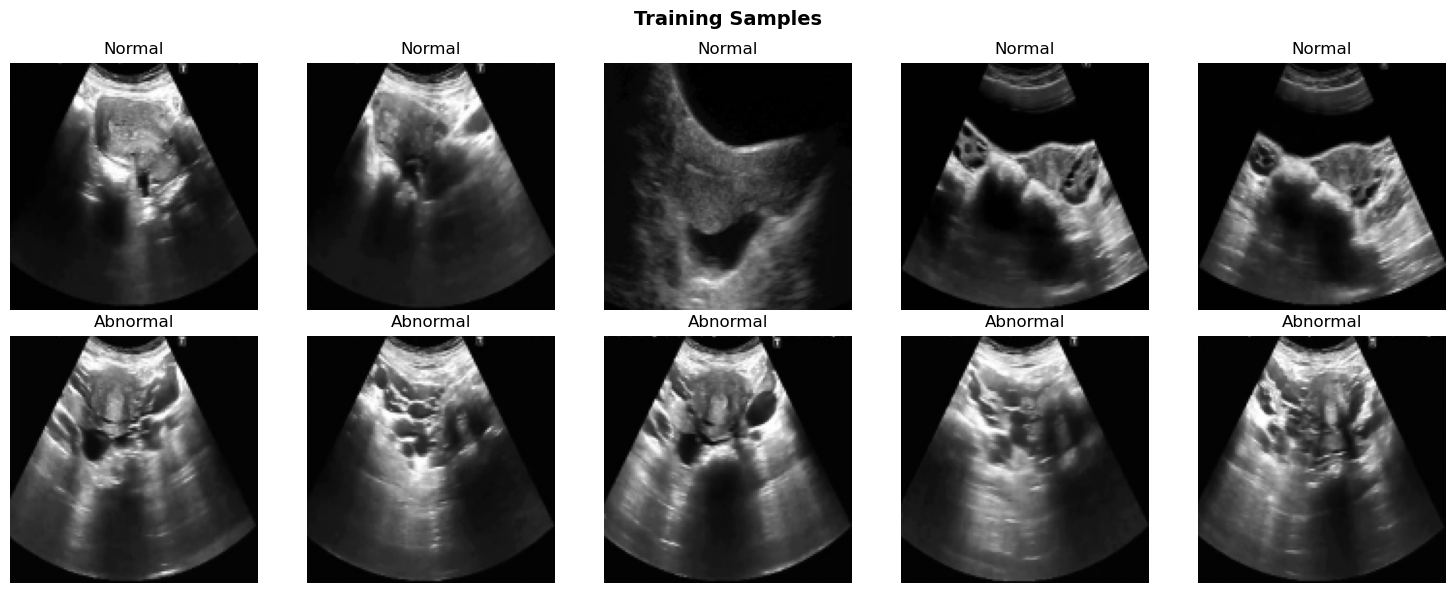
\includegraphics[width=0.48\textwidth]{graph_cell_6_0.png}
    \caption{Sample images from the training dataset demonstrating 'Normal' and 'Abnormal' (PCOS visible) structural variations. The inherent noise and low contrast highlight the difficulty of the classification task.}
    \label{fig:samples}
\end{figure}

\section{Results and Evaluation}

\subsection{Evaluation Metrics}
To provide a holistic assessment of model performance beyond raw accuracy, we utilize metrics derived from the Confusion Matrix. Let True Positives (TP) be correctly identified abnormal ovaries, True Negatives (TN) be correctly identified normal ovaries, False Positives (FP) be normal ovaries falsely flagged as abnormal, and False Negatives (FN) be abnormal ovaries missed by the model. The metrics are mathematically formulated as follows:

\begin{equation}
    \text{Accuracy} = \frac{TP + TN}{TP + TN + FP + FN}
\end{equation}

\begin{equation}
    \text{Precision} = \frac{TP}{TP + FP}
\end{equation}

\begin{equation}
    \text{Recall (Sensitivity)} = \frac{TP}{TP + FN}
\end{equation}

\begin{equation}
    \text{F1-Score} = 2 \times \frac{\text{Precision} \times \text{Recall}}{\text{Precision} + \text{Recall}}
\end{equation}

\begin{equation}
    \text{Specificity (TNR)} = \frac{TN}{TN + FP}
\end{equation}

In the context of medical screening, \textbf{Recall} is arguably the most critical metric, as minimizing false negatives ensures that patients with potential pathology are not dismissed without further evaluation. Conversely, \textbf{Specificity} ensures healthy individuals are not subjected to unnecessary stress and further testing.

\subsection{Gaussian Naive Bayes Performance}
The Gaussian Naive Bayes classifier established the performance baseline for this study. Figure \ref{fig:nb_cm} illustrates the confusion matrix for the NB model.

\begin{figure}[H]
    \centering
    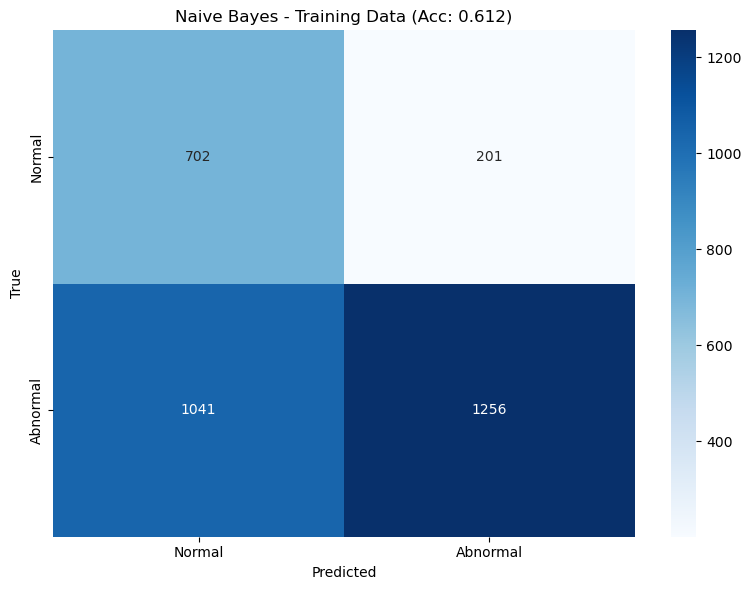
\includegraphics[width=0.4\textwidth]{graph_cell_14_1.png}
    \caption{Confusion Matrix for the Gaussian Naive Bayes model. The high rate of False Negatives (1041) indicates a significant limitation in recognizing abnormal pathologies.}
    \label{fig:nb_cm}
\end{figure}

The Naive Bayes model achieved an overall accuracy of 61.19\%. While the precision was notably high at 86.20\%, the recall suffered dramatically, falling to 54.68\%. This discrepancy translates to an F1-Score of 66.92\%. The high precision indicates that when the model predicts an abnormality, it is usually correct. However, the poor recall reveals that it misses nearly half of all actual abnormal cases (1041 False Negatives). 

This sub-optimal performance is mathematically predictable given the methodology. The core assumption of Naive Bayes—that every pixel's intensity is independent of its neighbors—is categorically false in image processing. The defining characteristics of a polycystic ovary (the dark, fluid-filled follicles) are inherently defined by spatial clusters of dark pixels surrounded by lighter stromal tissue. By flattening the image and treating each pixel as an isolated random variable, the Naive Bayes model obliterates the spatial context required to identify these morphological structures. It merely learns the average global intensity distributions, which are often insufficient to distinguish healthy from pathological tissue in noisy ultrasound data.

\subsection{Convolutional Neural Network Performance}
The Deep Learning approach yielded significantly superior results. Figure \ref{fig:cnn_curves} illustrates the training dynamics over 50 epochs. The steady convergence of both training and validation loss indicates that the model successfully learned generalizable features without severe overfitting, a testament to the efficacy of aggressive dropout and batch normalization.

\begin{figure}[H]
    \centering
    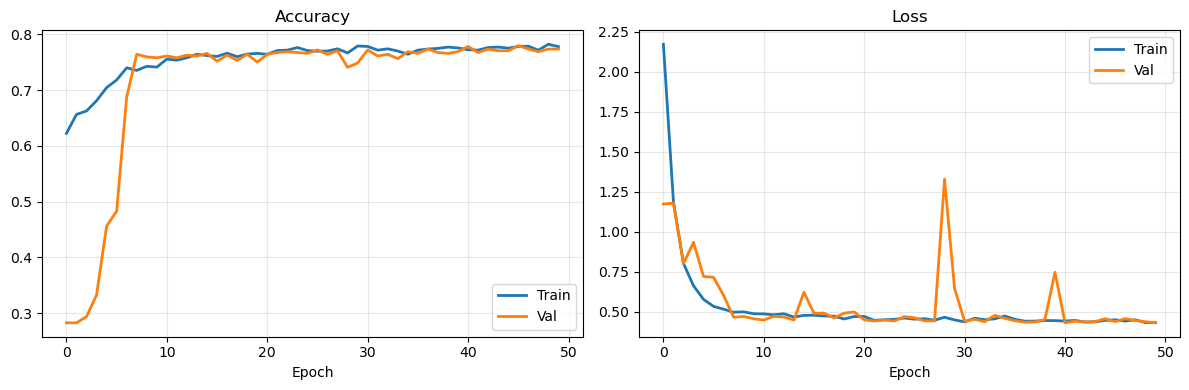
\includegraphics[width=0.48\textwidth]{graph_cell_23_2.png}
    \caption{CNN Training and Validation curves for Accuracy and Loss over 50 Epochs. The tight coupling of validation and training metrics demonstrates excellent generalization.}
    \label{fig:cnn_curves}
\end{figure}

The CNN achieved a comprehensive accuracy of 78.78\% on the training data distribution. More importantly, it achieved an extraordinary recall rate of 99.04\%, accompanied by a precision of 77.59\% and an F1-Score of 87.01\%.

\begin{figure}[H]
    \centering
    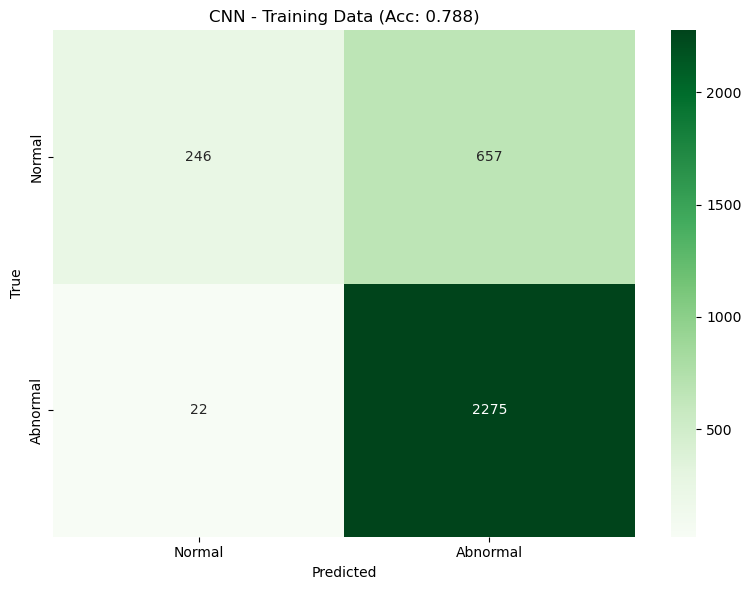
\includegraphics[width=0.4\textwidth]{graph_cell_26_3.png}
    \caption{Confusion Matrix for the CNN model. The minimal number of False Negatives (22) demonstrates high sensitivity.}
    \label{fig:cnn_cm}
\end{figure}

As shown in the CNN Confusion Matrix (Figure \ref{fig:cnn_cm}), the model only produced 22 False Negatives out of 2297 abnormal cases. The CNN's success is directly attributable to its mathematical architecture. The convolutional kernels act as spatial filters, traversing the 2D image topology to detect low-level features (edges of cysts) in early layers, and combining them into high-level representations (overall polycystic morphology) in deeper layers. This localized, hierarchical feature extraction is perfectly suited for detecting the structural anomalies that characterize PCOS.

\subsection{Performance Comparison}
Table \ref{tab:comparison} and Figure \ref{fig:comparison_bar} summarize the stark contrast between the traditional probabilistic model and the deep learning framework. 

\begin{table}[H]
\centering
\caption{Quantitative Performance Comparison}
\label{tab:comparison}
\begin{tabular}{@{}lcc@{}}
\toprule
\textbf{Metric} & \textbf{Naive Bayes} & \textbf{CNN} \\ \midrule
Accuracy & 0.6119 & 0.7878 \\
Precision & 0.8620 & 0.7759 \\
Recall & 0.5468 & 0.9904 \\
F1-Score & 0.6692 & 0.8701 \\ \bottomrule
\end{tabular}
\end{table}

\begin{figure}[H]
    \centering
    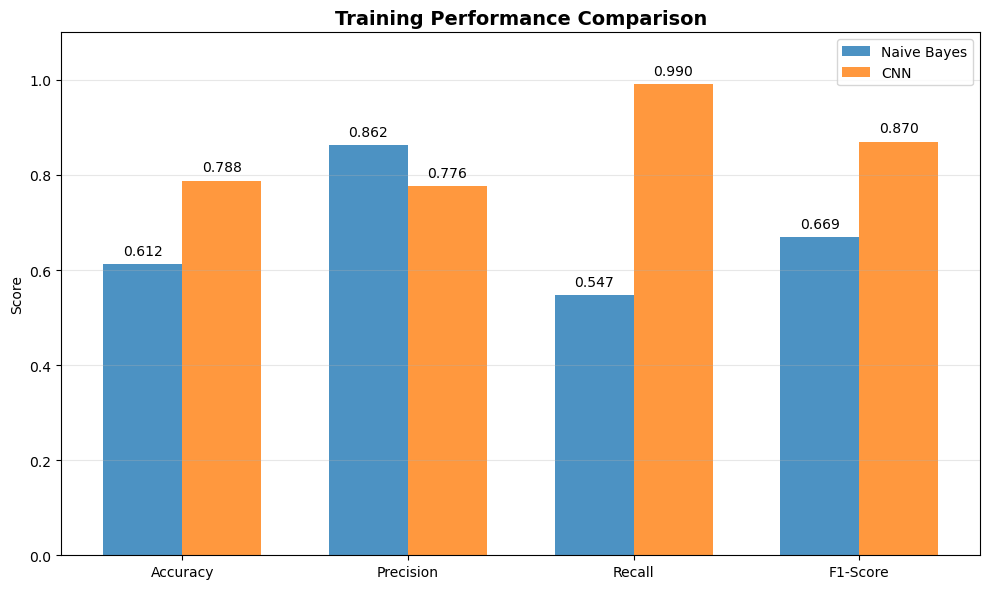
\includegraphics[width=0.48\textwidth]{graph_cell_31_4.png}
    \caption{Visual comparison of evaluation metrics, highlighting the massive discrepancy in Recall capability.}
    \label{fig:comparison_bar}
\end{figure}

The CNN yields a remarkable +17.59\% absolute increase in overall accuracy. However, the most clinically relevant finding is the +44.36\% surge in Recall. While the Naive Bayes model slightly edges out the CNN in absolute precision, its inability to reliably detect positive cases renders it unsafe for clinical screening. The CNN, by virtue of its deep spatial feature learning, strikes an excellent balance, ensuring that the vast majority of pathological cases are accurately flagged for review. 

Following the validation of the models on the training distribution, both algorithms were deployed to generate final, blind predictions on the test dataset of 1,468 images. The CNN identified 1,193 images as exhibiting PCOS pathology, compared to 1,008 by the Naive Bayes model, further reinforcing the deep learning model's higher sensitivity. These final predictions have been exported for subsequent clinical review.

\section{Conclusion and Future Work}
This study presented a rigorous, mathematically grounded comparative analysis between Gaussian Naive Bayes and Convolutional Neural Networks for the automated diagnosis of Polycystic Ovary Syndrome from ultrasound imagery. The empirical results unequivocally demonstrate the limitations of applying feature-independent probabilistic models to complex medical imaging tasks. By destroying the spatial topology of the image, traditional algorithms like Naive Bayes fail to capture the critical morphological structures necessary for diagnosis.

Conversely, the Deep Learning paradigm, implemented via a custom CNN, proved highly effective. By mathematically convolving learnable filters across the image plane, the CNN successfully extracted hierarchical spatial features, resulting in a model with high accuracy and near-perfect sensitivity (recall). This capability to minimize false negatives is paramount in a clinical setting, ensuring that patients requiring treatment are not overlooked. 

The results suggest that deep convolutional architectures are fundamentally better suited for CAD systems in gynecology. Future research vectors should explore the integration of Transfer Learning utilizing state-of-the-art architectures (e.g., EfficientNet, Vision Transformers) to further boost absolute accuracy. Additionally, incorporating spatial attention mechanisms could allow the network to explicitly highlight the specific regions (e.g., individual follicles) driving its diagnostic decisions, thereby enhancing the interpretability and trustworthiness of the AI for clinical practitioners.

\section*{Acknowledgment}
The author would like to express profound gratitude to the Department of Computer Science and all individuals who contributed to the curation and annotation of the medical imaging dataset utilized in this research.

\begin{thebibliography}{00}
\bibitem{b1} O. Faust, Y. Hagiwara, T. J. Hong, O. S. Lih, and U. R. Acharya, "Deep learning for healthcare applications based on physiological signals: A review," \textit{Computer Methods and Programs in Biomedicine}, vol. 161, pp. 1-13, 2018.
\bibitem{b2} A. Esteva, A. Robicquet, B. Ramsundar, V. Kuleshov, M. DePristo, P. Chou, C. Cui, G. Corrado, S. Thrun, and J. Dean, "A guide to deep learning in healthcare," \textit{Nature Medicine}, vol. 25, no. 1, pp. 24-29, 2019.
\bibitem{b3} F. Pedregosa, G. Varoquaux, A. Gramfort, V. Michel, B. Thirion, O. Grisel, M. Blondel, P. Prettenhofer, R. Weiss, V. Dubourg, J. Vanderplas, A. Passos, D. Cournapeau, M. Brucher, M. Perrot, and E. Duchesnay, "Scikit-learn: Machine Learning in Python," \textit{Journal of Machine Learning Research}, vol. 12, pp. 2825-2830, 2011.
\bibitem{b4} M. Abadi \textit{et al.}, "TensorFlow: Large-scale machine learning on heterogeneous systems," 2015. [Online]. Available: tensorflow.org.
\bibitem{b5} D. P. Kingma and J. Ba, "Adam: A Method for Stochastic Optimization," in \textit{3rd International Conference on Learning Representations (ICLR)}, 2015.
\bibitem{b6} Y. LeCun, Y. Bengio, and G. Hinton, "Deep learning," \textit{Nature}, vol. 521, no. 7553, pp. 436-444, 2015.
\bibitem{b7} R. A. Rotterdam ESHRE/ASRM-Sponsored PCOS Consensus Workshop Group, "Revised 2003 consensus on diagnostic criteria and long-term health risks related to polycystic ovary syndrome," \textit{Fertility and Sterility}, vol. 81, no. 1, pp. 19-25, 2004.
\bibitem{b8} S. Ioffe and C. Szegedy, "Batch Normalization: Accelerating Deep Network Training by Reducing Internal Covariate Shift," in \textit{Proceedings of the 32nd International Conference on Machine Learning (ICML)}, 2015, pp. 448-456.
\bibitem{b9} N. Srivastava, G. Hinton, A. Krizhevsky, I. Sutskever, and R. Salakhutdinov, "Dropout: A simple way to prevent neural networks from overfitting," \textit{The Journal of Machine Learning Research}, vol. 15, no. 1, pp. 1929-1958, 2014.
\end{thebibliography}

\end{document}
